\documentclass[class=article, crop=false]{standalone}

\begin{document}
\section{Partie 3 - Contrôleur}
\subsection{Question 11}
\begin{exercise}
    Le linéarisé tangent est-il commandable? Vérifier le rang de la matrice de commandabilité avec MATLAB. On pourra également s'assurer que la matrice de commandabilité est bien conditionnée.
\end{exercise}
\begin{resolution}
    On note que le système sera Commandable si et seulement si la Matrice de Commandabilité $\mathcal{C}(A, B)$:
    \begin{equation}
        \boxed{
            \mathcal{C}(A, B) = 
            \begin{bmatrix}
                B & A\times B & \cdots & A^{n-1}\times B
            \end{bmatrix}
        }
    \end{equation}
    est de rang dim$(x)$, c'est-à-dire: si la matrice $\mathcal{C}(A, B)$ a une numéro de colognes linéairement indépendants égale à dimension du vecteur des états $x$, le système est commandable.\\
    
    En utilisant le code suivant on calcule la matrice de Commandabilité:
    \begin{scriptsize}\mycode
        \lstinputlisting[language=Matlab]{../src/Q11.m}
    \end{scriptsize}
    \begin{scriptsize}\mycode
        \begin{lstlisting}[language=Matlab]
>>>
sucess: system controable, rank 4

COM =
            0         0         0 -272.5000
            0         0 -272.5000         0
            0   50.0000         0         0
      50.0000         0         0         0

cond(COM, 1) =
    5.4500
        \end{lstlisting}
    \end{scriptsize}
    Le système est défini avec 4 états et, comme on peut voir avec le résultat du code, le rank de la matrice de commandabilité est aussi 4, car elle a quatre 4 colognes linéairement indépendants, donc le système est commandable.\\

    On note aussi que \texttt{cond(COM, 1) = 5.45} qui est proche de 1 et donc indique une matrice bien conditionnée. 
    
    \begin{remark}
        Le \texttt{cond(COM, 1)} dépendra de la norme utilise comme donne par la définition: \texttt{cond(X, P) = NORM(X,P) * NORM(INV(X),P)}. Dans ce cas, la norme 1 a était considère.
    \end{remark}
\end{resolution}

\newpage
\subsection{Question 12}
On cherche tout d'abord à réaliser un bouclage d'état $\delta u(t) = - K \cdot \delta X(t)$ qui place les valeurs propres en boucle fermée en $-\omega$, $-2\omega$ et $-\omega \pm i\omega$.
\begin{exercise}
    Calculer dans MATLAB le gain K qui place les valeurs propres en boucle fermée sur les valeurs voulues. On pourra utiliser la fonction \href{https://www.mathworks.com/help/control/ref/place.html}{\texttt{place}}. Vérifier numériquement les valeurs propres en boucle fermée avec MATLAB.
\end{exercise}
\begin{resolution}
    En utilisant le code suivant on boucle les valeurs propres sur les valeurs voulues:
    \begin{scriptsize}\mycode
        \lstinputlisting[language=Matlab]{../src/Q12.m}
    \end{scriptsize}
    \begin{scriptsize}\mycode
        \begin{lstlisting}[language=Matlab]
>>>
success: closed-loop pole assignment

K =

  -29.4300   -9.3009    8.0098    0.6328
        \end{lstlisting}
    \end{scriptsize}
    Après avoir fait la verification les valeurs propres sont en effet en boucle fermée.
\end{resolution}

\newpage
\subsection{Question 13}
\begin{exercise}
    Implémenter dans le modèle Simulink le retour d'état  $\delta u(t) = -K \cdot \delta X(t)$ qui place les valeurs propres en boucle fermée sur les valeurs propres voulues.\\
    
Vérifier que le retour d'état permet bien de stabiliser la balle sur la position $r_{\text{ref}} = 0$ avec un état initial suffisamment proche de l'équilibre pour que le linéarise tangent reste une approximation valable.
\end{exercise}
\begin{resolution}
    Après avoir définit $K$ le système suivant a été mis en oeuvre sur Simulink:
    \begin{figure}[H]
        \centering
        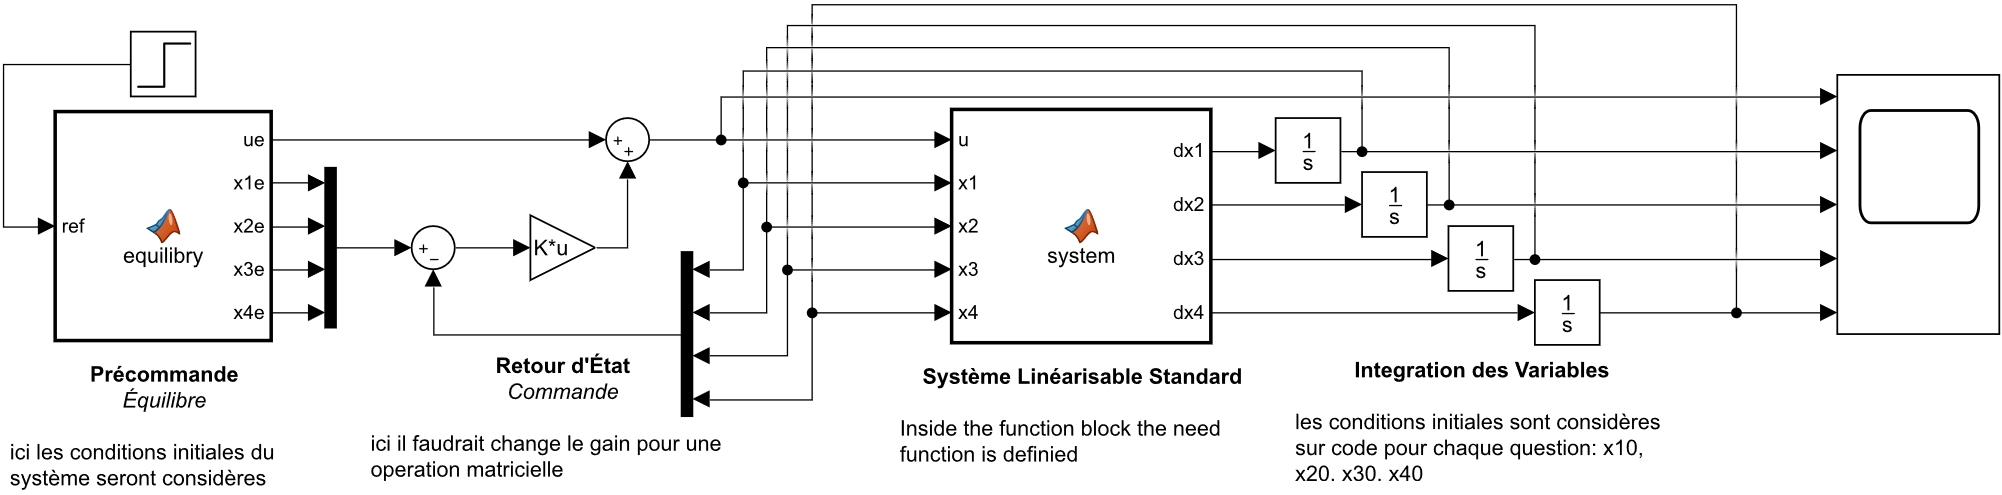
\includegraphics[width=0.8\textwidth]{../images/system_simulink_3.png}
        \caption{Système d'Intérêt Simulink, Retour d'État}
    \end{figure}
    Qui donne les résultats suivants:
    \begin{figure}[H]
        \centering
        \begin{subfigure}[b]{0.475\textwidth}
            \centering
            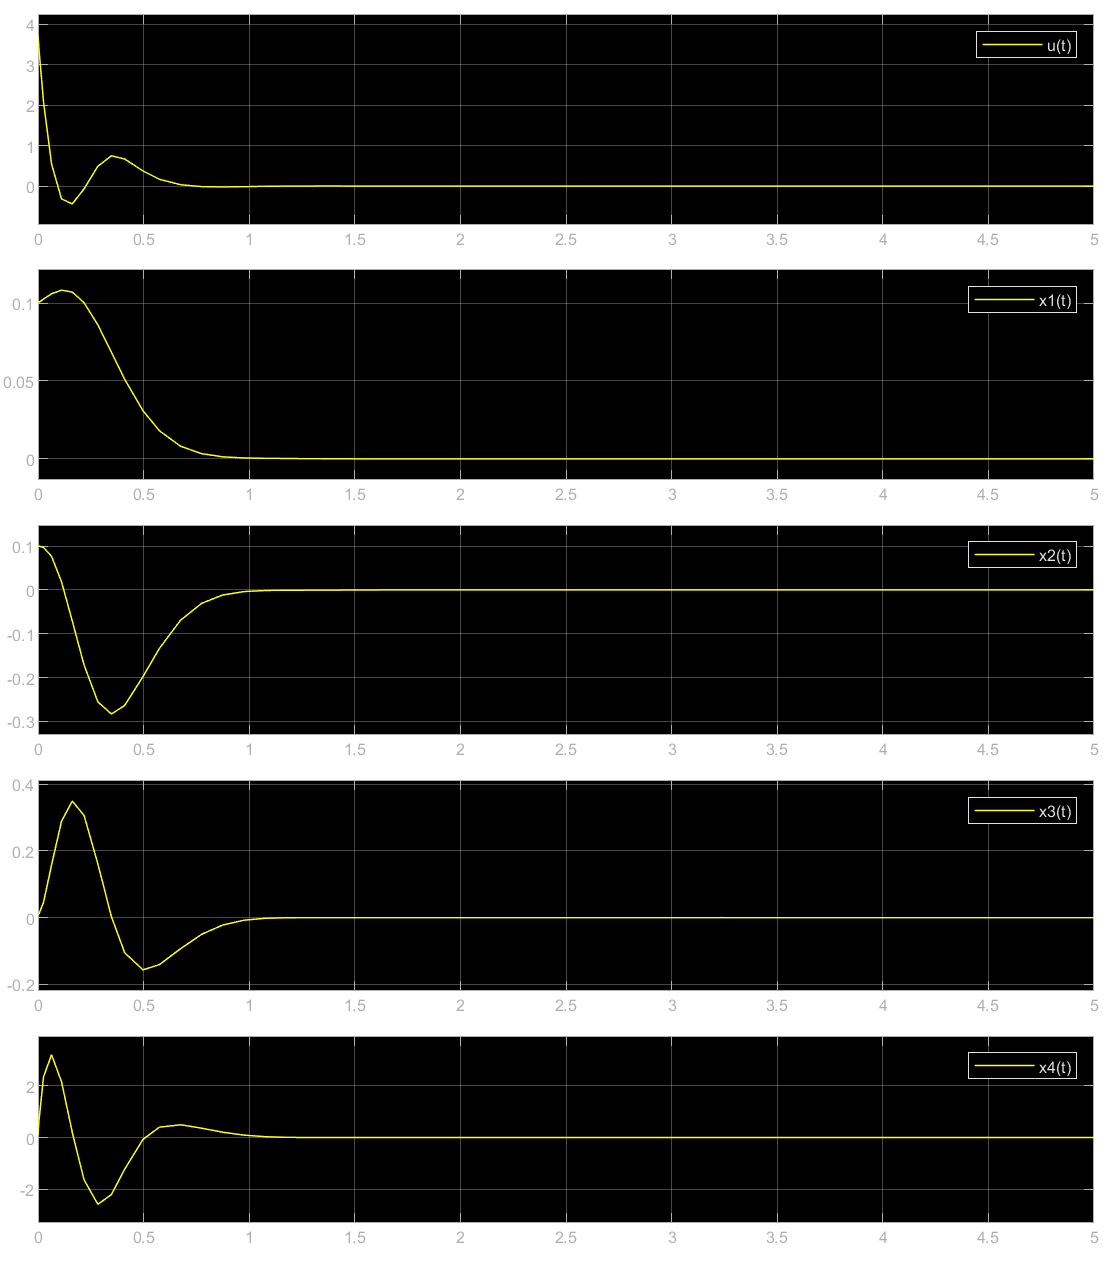
\includegraphics[width=\textwidth]{../images/simulink_scope3_0_01.png}
            \caption{$x_1(0) = x_2(0) = x_3(0) = x_4(0) = 0.1$}
        \end{subfigure}
        \begin{subfigure}[b]{0.475\textwidth}
            \centering
            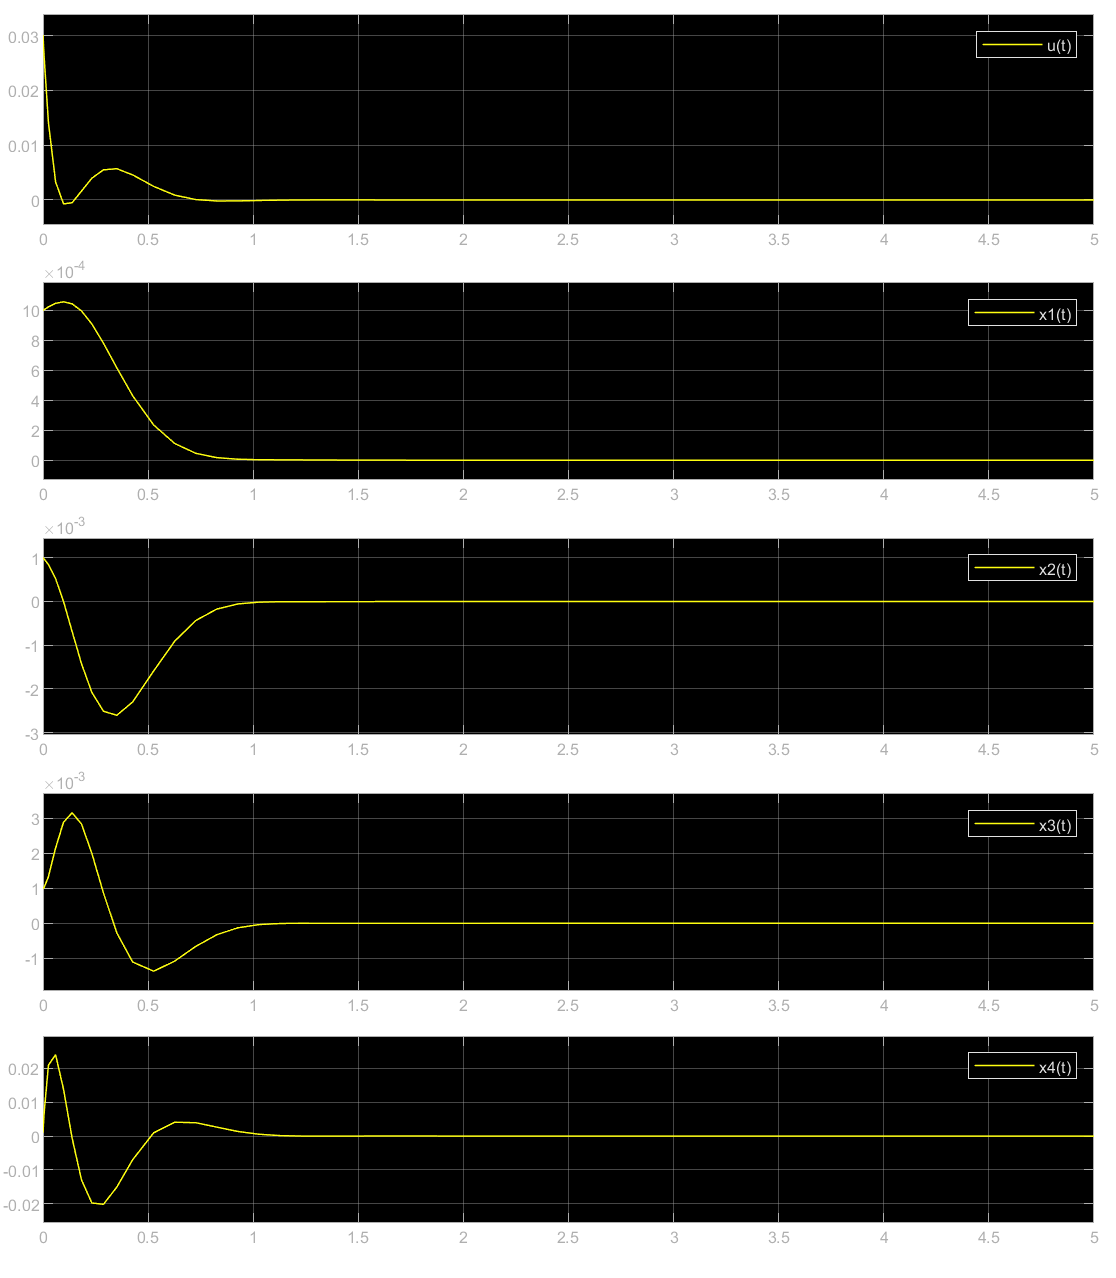
\includegraphics[width=\textwidth]{../images/simulink_scope3_0_001.png}
            \caption{$x_1(0) = x_2(0) = x_3(0) = x_4(0) = 0.001$}
        \end{subfigure}
        \caption{Simulation Retour d'État, Gain Voulue}
    \end{figure}
    On note que, proche des valeurs d'équilibre, le système converge à zéro.
\end{resolution}

\newpage
\subsection{Question 14}
On cherche maintenant à réaliser un bouclage d'état $\delta u(t) = -K \cdot X(t)$ qui minimise le critère:
\begin{equation}
    J_{LQ} = \frac{1}{2} \int^{\infty}_{0}
    ( \delta x^2_1(t) + \delta x^2_2(t) + \delta x^2_3(t) + \delta x^2_4(t) + \delta u^2(t)) \; \text{dt}
\end{equation}
\begin{exercise}
    Montrer que le critère $J_{LQ}$ peut s'écrire sous la forme:
    \begin{equation}
        J_{LQ} = \frac{1}{2} \int^{\infty}_{0}
        ( \delta X^T(t) \; R \; \delta X(t) + \delta u(t) \; Q \; \delta u(t)) \; \text{dt}
    \end{equation}
    Identifier les matrices R et Q. Montrer que ce problème de commande optimale admet une solution. Rappeler comment est défini le gain optimal $K$.
\end{exercise}
\begin{resolution}
    On rappelle que la matrice des états $\delta X(t)$ a des dimensions $4\times 1$ et que la matrice d'entrée $\delta u(t)$ a des dimensions $1\times 1$ donc le système précédemment pourrait être écrit comme:
    \begin{equation*}
        ( 
            \underbrace{\delta X^T(t)}_{1\times 4}
            \; 
            {R}_{n\times n}
            \;
            \underbrace{\delta X(t)}_{4\times 1}
            + 
            \underbrace{\delta u(t)}_{1\times 1}
            \;
            {Q}_{m\times m}
            \;
            \underbrace{\delta u(t)}_{1\times 1}
        )
    \end{equation*}
    On note que la seule façon d'avoir $\delta u^2(t)$ c'est si $Q_{1\times 1} = 1$ et, par consequence, la seule façon d'avoir $\delta x^2_1(t) + \delta x^2_2(t) + \delta x^2_3(t) + \delta x^2_4(t)$ c'est si $R_{4\times 4} = I_{4\times 4}$.
    % TODO search definition of LQ
    % TODO do calculation
\end{resolution}

\newpage
\subsection{Question 15}
\begin{exercise}
    Calculer dans MATLAB le gain optimal K qui minimise le critère $J_{LQ}$. On pourra utiliser la fonction \href{https://www.mathworks.com/help/control/ref/lti.lqr.html}{\texttt{lqr}}. Quels sont les valeurs propres en boucle fermée?
\end{exercise}
\begin{resolution}
    En utilisant le code suivant calcule le gain optimal qui minimise le critère $J_{LQ}$:
    \begin{scriptsize}\mycode
        \lstinputlisting[language=Matlab]{../src/Q15.m}
    \end{scriptsize}
    En considerant $Q = I_{4x4}$ et $R = 1$ on a:
    \begin{scriptsize}\mycode
        \begin{lstlisting}[language=Matlab]
>>>
K =

  -11.8563   -4.0213    6.9244    1.1300
        \end{lstlisting}
    \end{scriptsize}
    \begin{remark}
        La nomenclature utilise pour la fonction sur MATLAB est différent de la nomenclature utilise sur le système.
    \end{remark}
\end{resolution}

\newpage
\subsection{Question 16}
\begin{exercise}
    Implémenter dans le modèle Simulink le retour d'état $\delta u(t) = - K \cdot \delta X(t)$ qui minimise le critère $J_{LQ}$. Vérifier que le retour d'état permet bien de stabiliser la Balle sur la position $r_{\text{ref}} = 0$ avec un état initial suffisamment proche de l'équilibre pour que le linéarise tangent reste une approximation valable.
\end{exercise}
\begin{resolution}
    Après avoir définit $K_{o}$ le gain optimale, le système suivant a été mis en oeuvre sur Simulink:
    \begin{figure}[H]
        \centering
        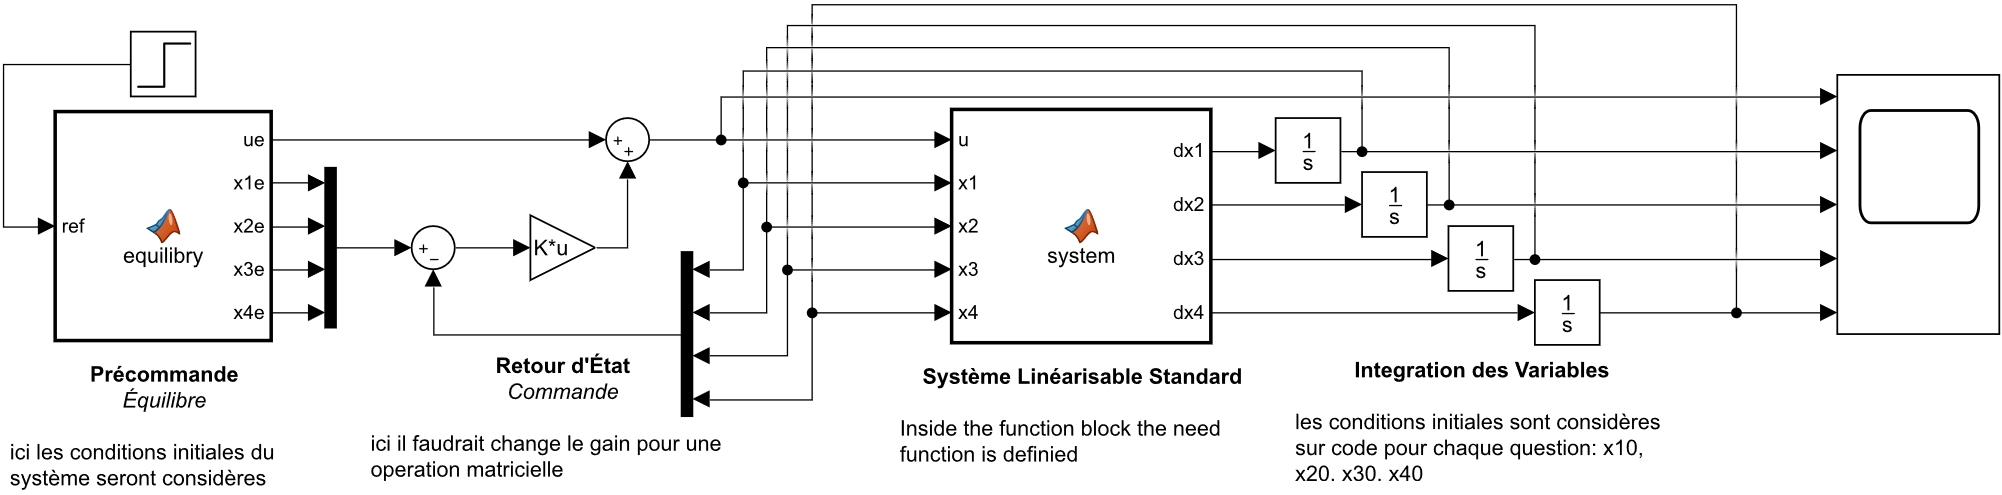
\includegraphics[width=0.8\textwidth]{../images/system_simulink_3.png}
        \caption{Système d'Intérêt Simulink, Retour d'État}
    \end{figure}
    Qui donne les résultats suivants:
    \begin{figure}[H]
        \centering
        \begin{subfigure}[b]{0.475\textwidth}
            \centering
            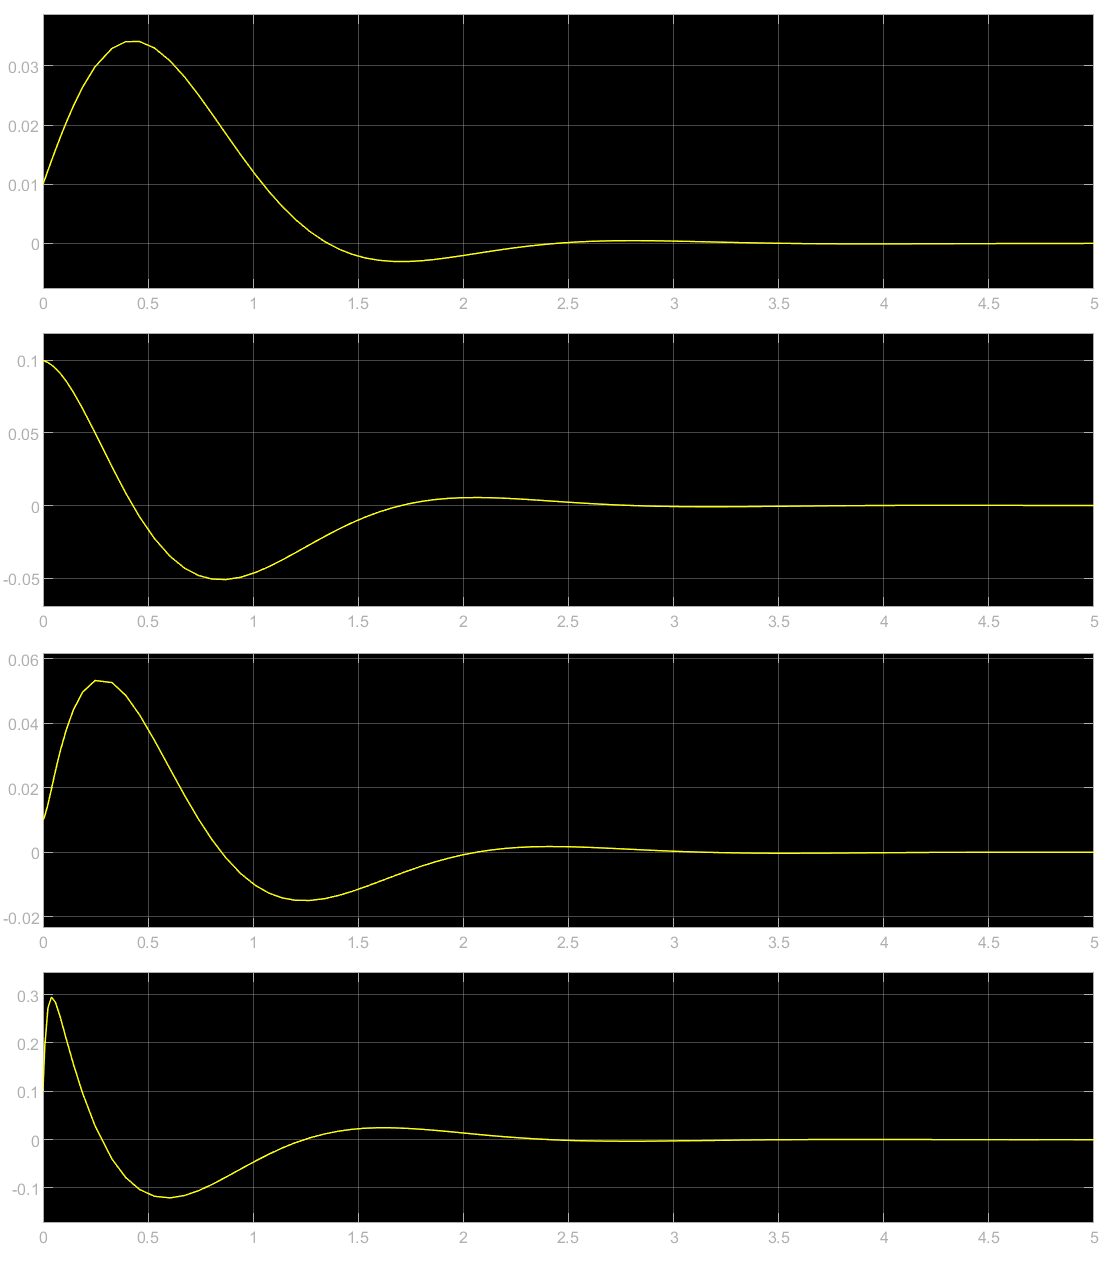
\includegraphics[width=\textwidth]{../images/simulink_scope3_0_01_1.png}
            \caption{$x_1(0) = x_2(0) = 0.01$ et $x_3(0) = x_4(0) = 0.1$}
        \end{subfigure}
        \begin{subfigure}[b]{0.475\textwidth}
            \centering
            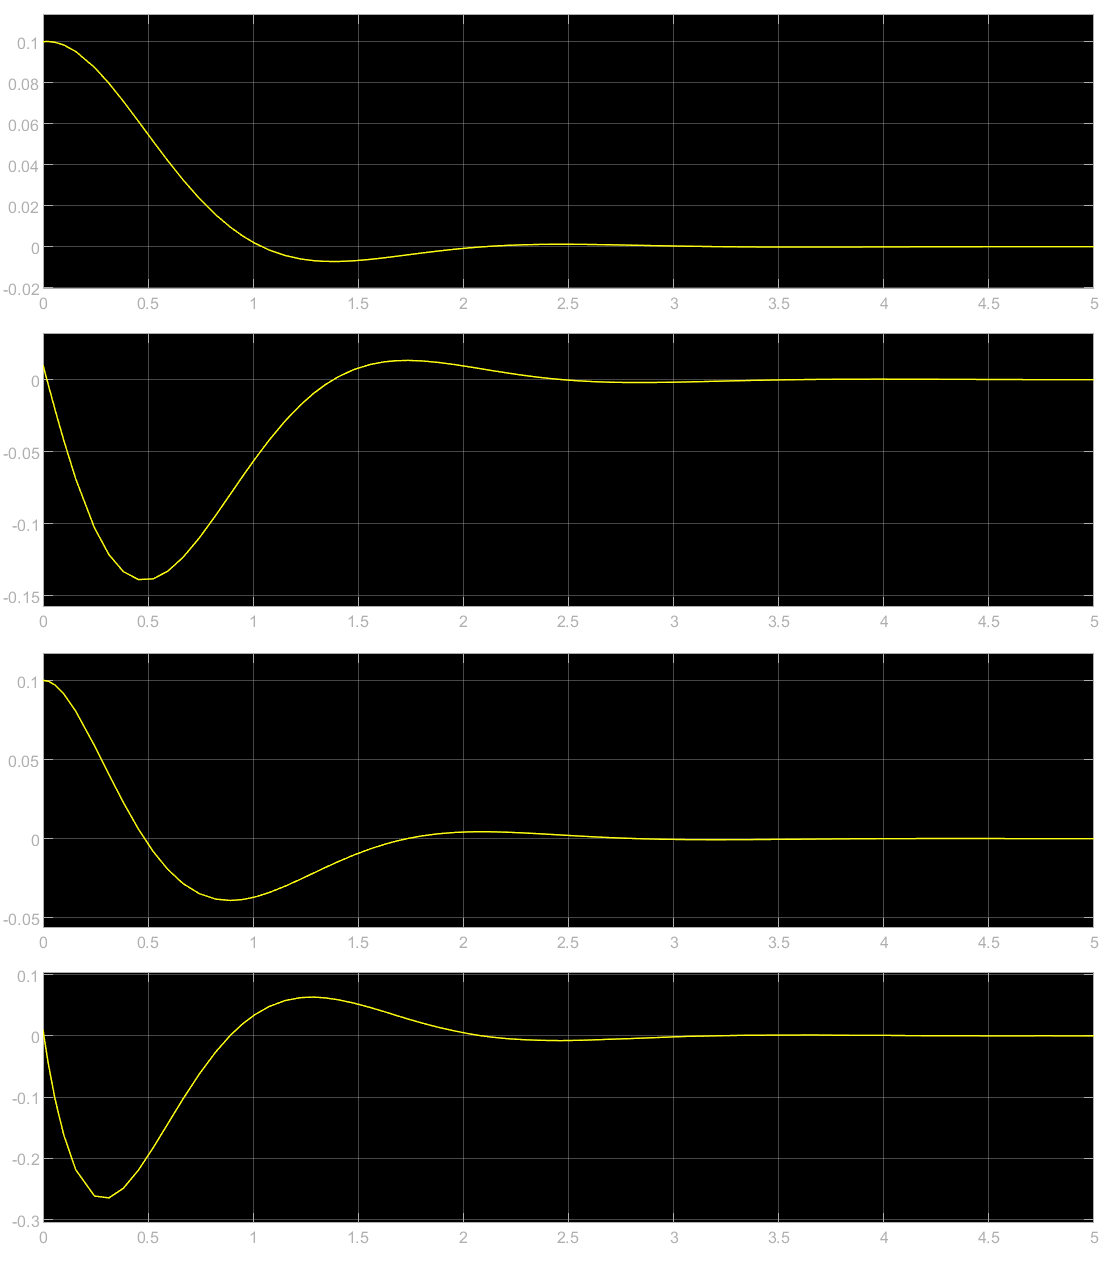
\includegraphics[width=\textwidth]{../images/simulink_scope3_0_1_01.png}
            \caption{$x_1(0) = x_2(0) = 0.1$ et $x_3(0) = x_4(0) = 0.01$}
        \end{subfigure}
        \caption{Simulation Retour d'État, Gain Optimale}
    \end{figure}
\end{resolution}

\newpage
\subsection{Question 17}
\begin{exercise}
    Comparer les résultats obtenus avec les deux méthodes.
\end{exercise}
\begin{resolution}
    Après avoir définit $K_{\omega}$, le gain voulue, $K_{o}$ le gain optimale, le système suivant a été mis en oeuvre sur Simulink:
    \begin{figure}[H]
        \centering
        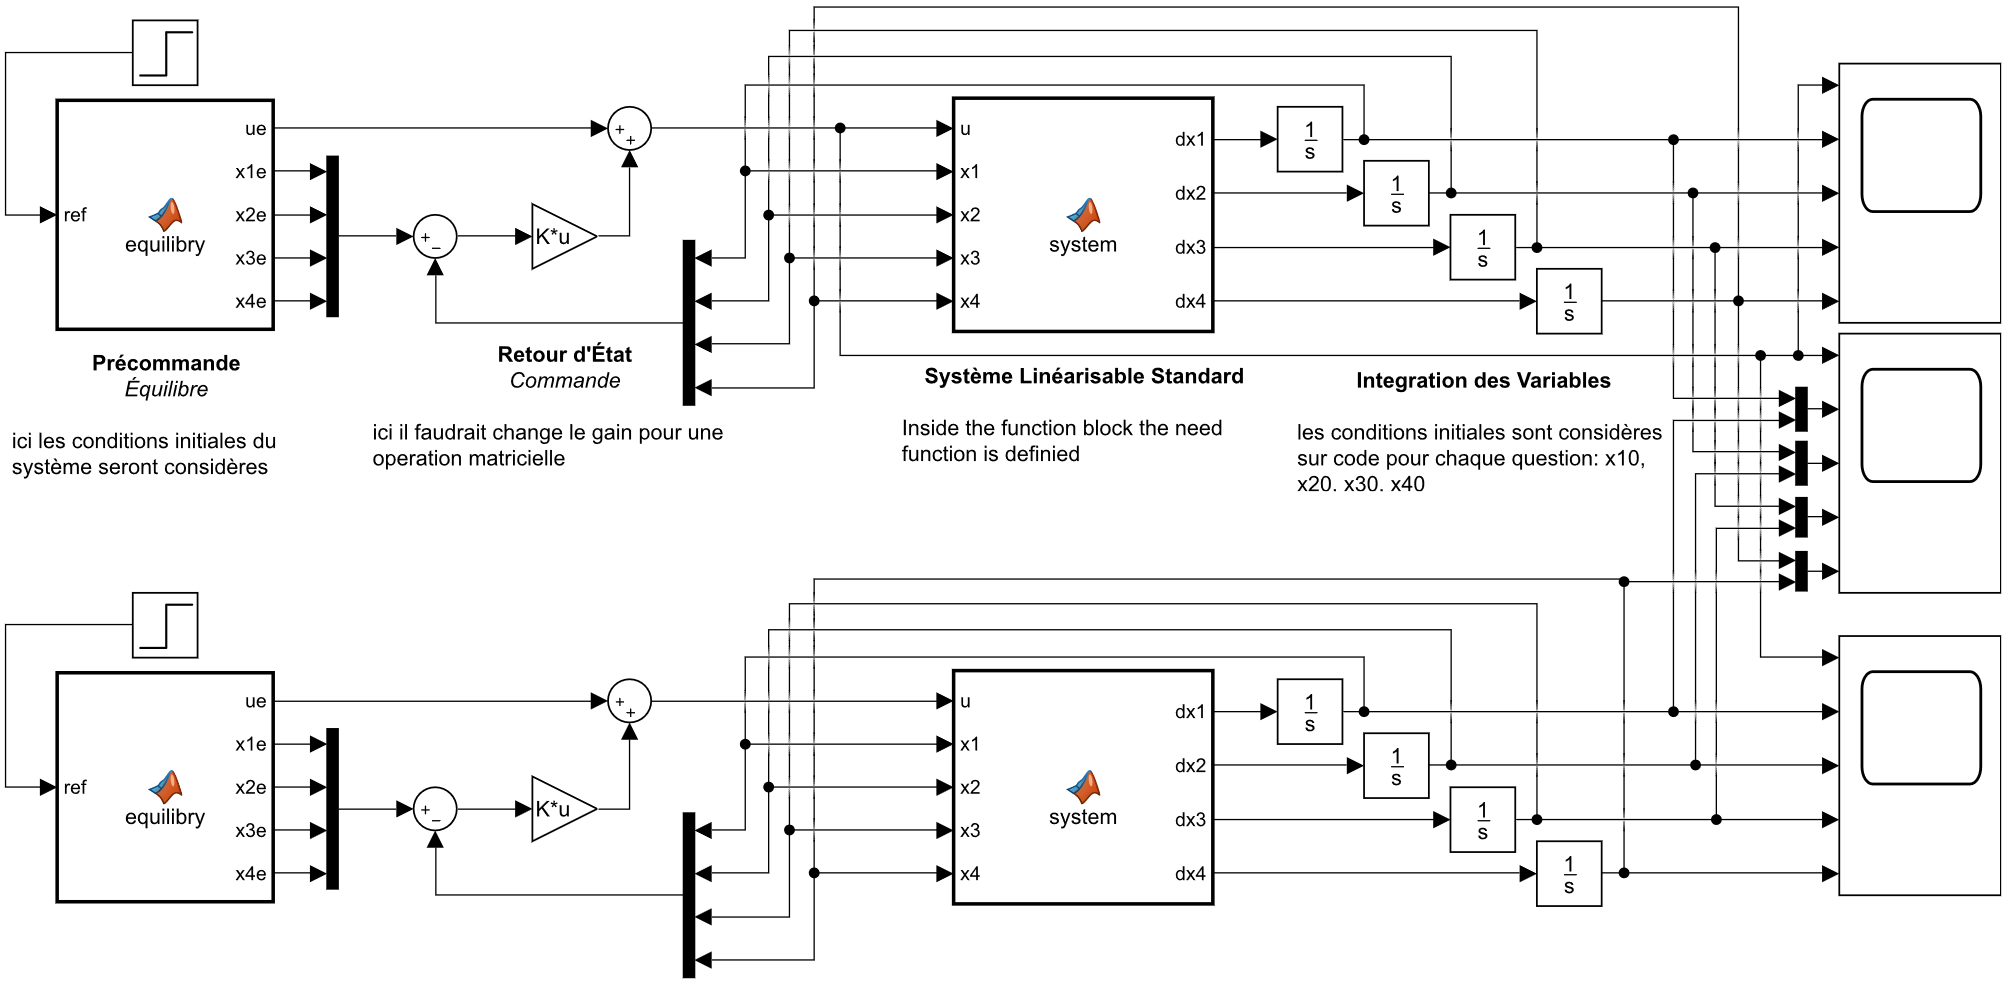
\includegraphics[width=0.8\textwidth]{../images/system_simulink_30.png}
        \caption{Système d'Intérêt Simulink, Retour d'État}
    \end{figure}
    Qui donne les résultats suivants:
    \begin{figure}[H]
        \centering
        \begin{subfigure}[b]{0.475\textwidth}
            \centering
            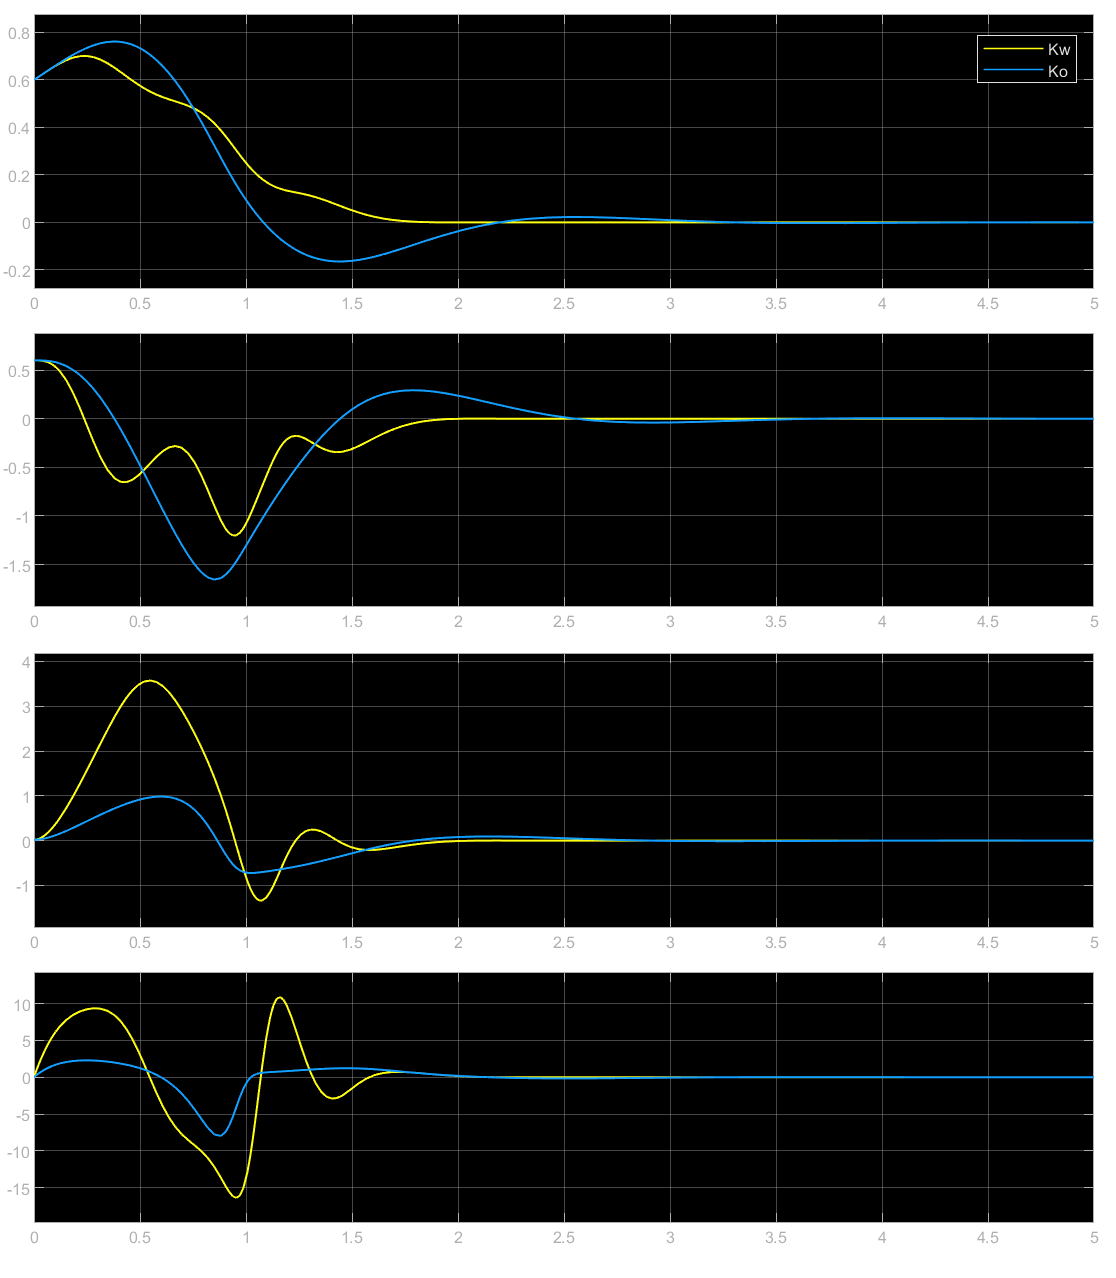
\includegraphics[width=\textwidth]{../images/simulink_scope30_0_6_02.png}
            \caption{$x_1(0) = x_2(0) = 0.6$ et $x_3(0) = x_4(0) = 0.02$}
        \end{subfigure}
        \begin{subfigure}[b]{0.475\textwidth}
            \centering
            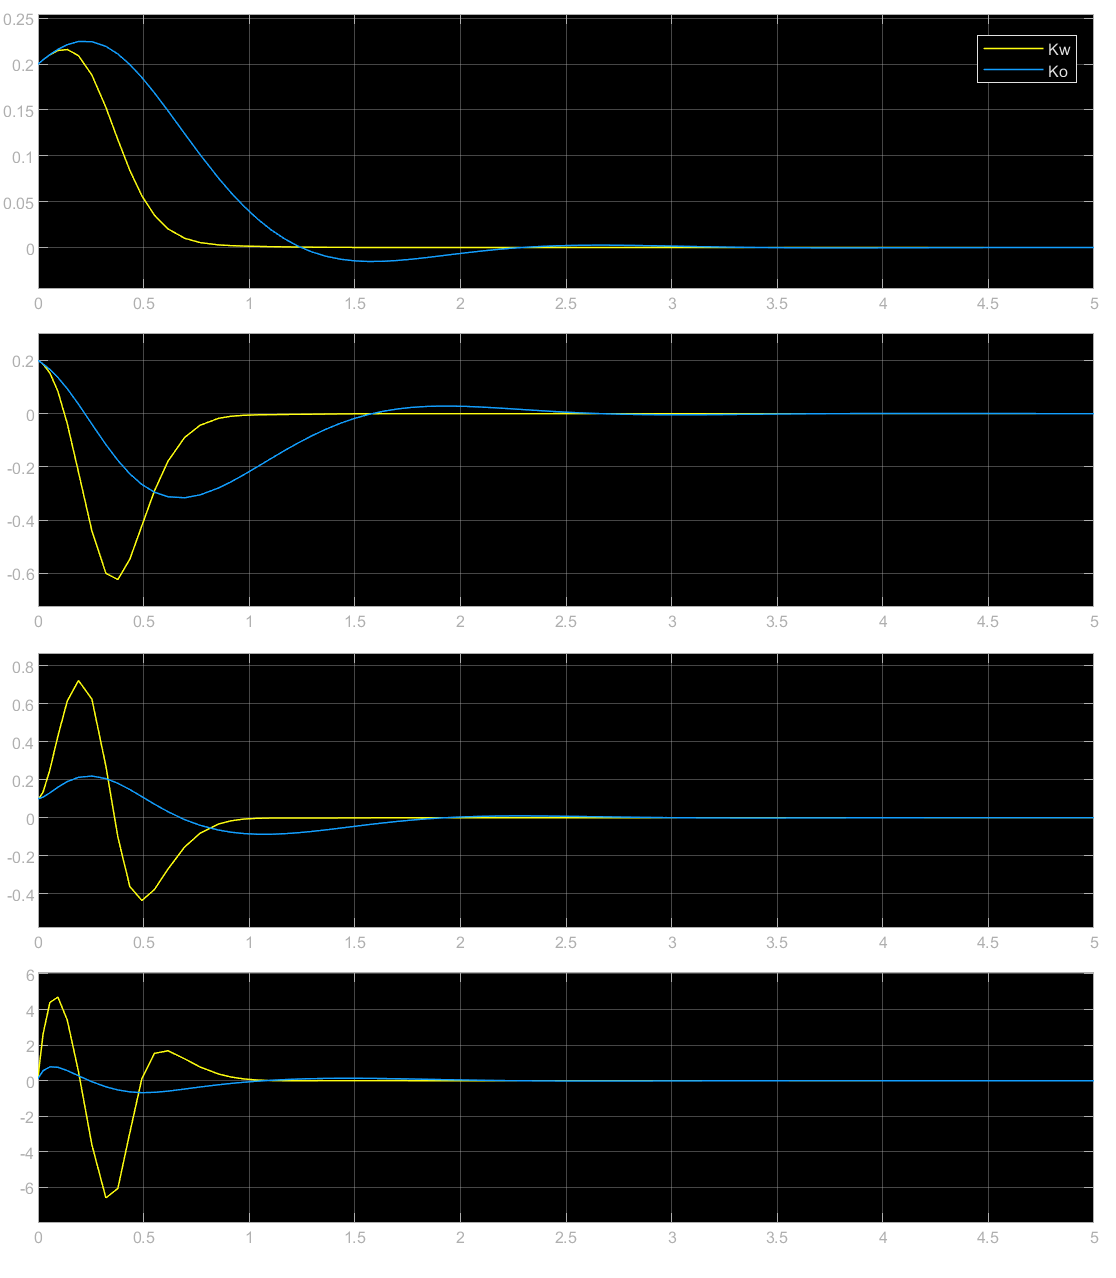
\includegraphics[width=\textwidth]{../images/simulink_scope30_0_02.png}
            \caption{$x_1(0) = x_2(0) = x_3(0) = x_4(0) = 0.02$}
        \end{subfigure}
        \caption{Simulation Retour d'État, Comparaison Gain}
    \end{figure}
    On peut voir que les résultats sont..\\
    % TODO compare results for different values
    % TODO estimate different poles and after compare with the optimal ones
    En tout cas, le méthode \href{https://www.mathworks.com/help/control/ref/lti.lqr.html}{\texttt{lqr}} permette de découvrir les poles plus facilement que le méthode de placement de pôle car le premier utilise d'une critère plus facile à comprendre, bénéficie ou pénaliser la variation des paramètres dans le système.
\end{resolution}
\end{document}